\documentclass{beamer}
%\documentclass[handout]{beamer}
\usepackage[hungarian]{babel}
\uselanguage{hungarian}
\languagepath{hungarian}
\deftranslation[to=hungarian]{Theorem}{T\'etel}
\deftranslation[to=hungarian]{Example}{P\'elda}
\deftranslation[to=hungarian]{Definition}{Defin\'ici\'o}
%\usepackage[magyar]{babel}
\usepackage[utf8]{inputenc}
\usepackage[T1]{fontenc}
\usepackage{beamerthemesplit}
\usepackage{pgf,pgffor,pgfplots}
\pgfplotsset{compat=1.15}
\usepackage{subfig}
\usepackage{xcolor}
\usepackage{listings}
\usepackage{nccfoots}
\newcommand{\framenote}[1]{%
  \Footnotetext{}{\emph{#1}}% Print footnote text
}

\makeatletter
\let\old@lstKV@SwitchCases\lstKV@SwitchCases
\def\lstKV@SwitchCases#1#2#3{}
\makeatother
\usepackage{lstlinebgrd}
\AtBeginEnvironment{figure}{\setcounter{subfigure}{0}}
\makeatletter
%%%%%%%%%%%%%%%%%%%%%%%%%%%%%%%%%%%%%%%%%%%%%%%%%%%%%%%%%%%%%%%%%%%%%%%%%%%%%%
%
% \btIfInRange{number}{range list}{TRUE}{FALSE}
%
% Test in int number <number> is element of a (comma separated) list of ranges
% (such as: {1,3-5,7,10-12,14}) and processes <TRUE> or <FALSE> respectively

\newcount\bt@rangea
\newcount\bt@rangeb

\newcommand\btIfInRange[2]{%
    \global\let\bt@inrange\@secondoftwo%
    \edef\bt@rangelist{#2}%
    \foreach \range in \bt@rangelist {%
        \afterassignment\bt@getrangeb%
        \bt@rangea=0\range\relax%
        \pgfmathtruncatemacro\result{ ( #1 >= \bt@rangea) && (#1 <= \bt@rangeb) }%
        \ifnum\result=1\relax%
            \breakforeach%
            \global\let\bt@inrange\@firstoftwo%
        \fi%
    }%
    \bt@inrange%
}
\newcommand\bt@getrangeb{%
    \@ifnextchar\relax%
        {\bt@rangeb=\bt@rangea}%
        {\@getrangeb}%
}
\def\@getrangeb-#1\relax{%
    \ifx\relax#1\relax%
        \bt@rangeb=100000%   \maxdimen is too large for pgfmath
    \else%
        \bt@rangeb=#1\relax%
    \fi%
}

%%%%%%%%%%%%%%%%%%%%%%%%%%%%%%%%%%%%%%%%%%%%%%%%%%%%%%%%%%%%%%%%%%%%%%%%%%%%%%
%
% \btLstHL<overlay spec>{range list}
%
% TODO BUG: \btLstHL commands can not yet be accumulated if more than one overlay spec match.
% 
\newcommand<>{\btLstHL}[1]{%
  \only#2{\btIfInRange{\value{lstnumber}}{#1}{\color{orange!30}\def\lst@linebgrdcmd{\color@block}}{\def\lst@linebgrdcmd####1####2####3{}}}%
}%
\makeatother

\usepackage{hyperref}
\hypersetup{
    colorlinks = true,
    linkcolor = blue,
    urlcolor  = blue,
    citecolor = blue,
    linkbordercolor = {white},
}
\usepackage{alltt}
\usepackage{tikz}
\usetikzlibrary{trees}
\usetikzlibrary{shapes,shapes.geometric,shapes.multipart}
\usetikzlibrary{calc,chains,arrows,positioning}
\tikzset{
  box/.style={draw, fill=pink!10, minimum width=5em, text centered, minimum 
  height=2.5em},
  treenode/.style = {circle, draw, align=center, inner sep=3pt, text centered, 
  font=\sffamily, text width=1em},
  int/.style = {rectangle split,rectangle split parts=2,draw,text centered, 
  text width = 1.6cm, text height = 0.3cm},
  subtree/.style={isosceles triangle, draw=black, align=center, shape border 
  rotate=90, anchor=north},
  data/.style={
	minimum width=2em,
	minimum height=2em,
	draw, rectangle split,
	rectangle split parts=2, text centered,
	}
}
\usetheme{Warsaw}
\institute{Szegedi Tudományegyetem}
\pgfdeclareimage[height=0.55cm]{institution-logo}{../szte_logo}
\logo{\pgfuseimage{institution-logo}}

\title{Algoritmusok és adatszerkezetek II.}
\subtitle{Kupacok}
\date{}

\begin{document}

\maketitle

\begin{frame}{Fapacok (Treaps)}
	\begin{block}{Emlékeztető}
		$n$ kulcsból álló \textbf{véletlen} építésű bináris keresőfa $h$ magasságának \textbf{várható értéke} $\log n$
	\end{block}
	\begin{itemize}
		\item Adverzaliális műveleti sorrend mellett azonban $n$ magas is lehet
	\end{itemize}
	\begin{alertblock}{Ötlet}
		A keresőfa,-és kupactulajdonságot egyidejűleg követeljük meg
		\begin{enumerate}
			\item Keresőfa tulajdonság biztosítja a kulcsok $O(h)$ kereshetőségét
			\item Kupactulajdonság miatt $h$ \textbf{várható értékben} $\log n$
			\begin{itemize}
				\item<2> A kupactulajdonság ne az eltárolt kulcsokra, hanem egy \textbf{véletlenszerűen} generált kiegészítőinformációra teljesüljön!
			\end{itemize}
		\end{enumerate}
	\end{alertblock}
\end{frame}

\begin{frame}{Kupacok}
   \begin{alertblock}{Felhasználásuk}
	\begin{enumerate}
		\item Prioritási sor megvalósításánál fontos, hogy a minimális/maximális kulcsot hatékonyan tudjuk visszaadni
		\item Szintén fontos művelet egy adott kulcs értékének módosítása
	\end{enumerate}
   \end{alertblock}

\pause
   \begin{block}{Kupactulajdonság}
   	Azt mondjuk, hogy egy fa rendelkezik a minimum (maximum) kupactulajdonsággal, ha minden $p$ csúcsának minden $q$ fiára
   	\begin{itemize}
   		\item $q=Nil$ vagy
   		\item $p.kulcs < q.kulcs$ ($p.kulcs > q.kulcs$)
   	\end{itemize}
   \end{block}
\end{frame}

\begin{frame}{Példa maximum bináris kupacra}
	\begin{columns}
		\begin{column}{.3\linewidth}
			\begin{tikzpicture}[sibling distance=2cm]
			\node[circle,draw]{33}
			child{
				node[circle,draw]{22}
				child[sibling distance=1cm]{node[circle,draw]{11}}
				child[sibling distance=1cm]{node[circle,draw]{15}}}
			child{node[circle,draw]{12}
			};
			\end{tikzpicture}
			\begin{tabular}{|c|c|c|c|c|c|}
				\hline
				0&1&2&3&4&5 \\ \hline
				--&33&22&12&11&15\\ \hline
			\end{tabular}
		\end{column}
		\begin{column}{.1\linewidth}
			{\scshape Beszúr(40)}
		\end{column}
		\begin{column}<2->{.5\linewidth}
		\begin{tikzpicture}[sibling distance=2cm]
		\node[circle,draw]{40}
		child{
			node[circle,draw]{22}
			child[sibling distance=1cm]{node[circle,draw]{11}}
			child[sibling distance=1cm]{node[circle,draw]{15}}}
		child{node[circle,draw]{33}
			child[sibling distance=1cm]{node[circle,draw]{12}}
			child[missing]
		};
		\end{tikzpicture}
			\begin{tabular}{|c|c|c|c|c|c|c|}
			\hline
			0&1&2&3&4&5&6 \\ \hline
			--&40&22&33&11&15&12\\ \hline
			\end{tabular}
		\end{column}
	\end{columns}
	\begin{block}{Bináris kupac}
		\textbf{Teljes} bináris fa, melyre teljesül a kupactulajdonság. \\
		$\Rightarrow$ mivel legfeljebb egy belső pontnak lehet 2-nél kevesebb fia, így egyszerűen egy tömbbel implementálhatjuk
	\end{block}
\end{frame}

\begin{frame}{Fapac példa}
\begin{columns}
	\begin{column}{.3\linewidth}
		\begin{tikzpicture}
		\node[data]{15 \nodepart{two} \textcolor{red}{80}}
		child{
			node[data]{12 \nodepart{two} \textcolor{red}{74}}
			child{node[data]{11 \nodepart{two} \textcolor{red}{21}}}
			child[missing]}
		child{node[data]{22 \nodepart{two} \textcolor{red}{61}}
			child[missing]
			child{node[data]{33 \nodepart{two} \textcolor{red}{10}}}
		};
		\end{tikzpicture}
	\end{column}

	\begin{column}{.7\linewidth}
		\begin{itemize}
			\item A kulcsok keresőfa tulajdonság szerint helyezkednek el
			\item A véletlen felépítést az \textcolor{red}{extra adattag} eredményezi
			\item A kiegyensúlyozott fáknál megszokott módon állítjuk helyre a megkövetelt tulajdonságokat (pl.~{\scshape(Beszúr(27, \textcolor{red}{100}))})
		\end{itemize}
	\end{column}
\end{columns}
\end{frame}

\begin{frame}{Vissza a kupacokhoz}
	\begin{tabular}{@{}ll@{}}
	$n$ elemű kupacban hogy keresnénk meg a maximális elemet? &
	\only<2>{$O(1)$} \\
	És egy adott kulcs rákövetkezőjét? & \only<2>{$O(n)$} \\
	Hogy egyesítenénk egy $n_1$ és egy $n_2$ kulcsból álló kupacot? 
	& \only<2>{$O(n_1+n_2)$} \\
	\end{tabular}
	\begin{block}<2>{Kérdés}
	Lehetne hatékonyabban is?
	\end{block}
\end{frame}

\section{Binomiális kupacok}

\begin{frame}{Binomiális fa}
\begin{definition}
$B_k$ binomiális fa egy rekurzív rendezett fa, amely két 
összekapcsolt $B_{k-1}$ binomiális fából áll; az egyik fa gyökércsúcsa a másik 
fa gyökércsúcsának legbaloldalibb gyereke
\end{definition}

\begin{columns}[T]
	\begin{column}{.2\linewidth}
		\begin{block}{$B_0$}
			\begin{tikzpicture}
				\node[treenode,minimum width=.7cm]{};
			\end{tikzpicture}
		\end{block}
	\end{column}
	\begin{column}{.4\linewidth}
		\begin{block}{$B_k (k \geq 1)$}
			\begin{tikzpicture}
				\node[draw,circle,minimum 
				width=.7cm,xshift=2cm,yshift=1cm](A){}{node[subtree,xshift=2cm,yshift=1cm]{$B_{k-1}$}};
				\node[draw,circle,minimum 
			width=.7cm](B){}{node[subtree]{$B_{k-1}$}};
				\draw(A)--(B);
			\end{tikzpicture}
		\end{block}
	\end{column}
\end{columns}
\end{frame}

\begin{frame}{Binomiális fákkal kapcsolatos állítások}
	\begin{lemma}{}
		Ha $B_k$ binomiális fa, akkor az alábbi állítások teljesülnek:
		\begin{enumerate}
			\item $2^k$ csúcsa van
			\item $i$-edik mélységében pontosan $\binom{k}{i}$ csúcs van 
			($i=0,1,\ldots, k$)
			\item a gyökércsúcs fokszáma (fokszám helyett találkozhatunk a 
			rang, illetve rend kifejezésekkel is) $k$, melynek 	gyerekeit 
			balról jobbra megszámozva $k-1, k-2, \ldots, 0$-al, $i$-dik gyereke 
			egy $B_i$ részfa gyökércsúcsa.
		\end{enumerate}
	\end{lemma}
	
	\begin{alertblock}<2>{Következmény}
    $n$ csúcsú binomiális fa minden csúcsának fokszáma legfeljebb $\log{n}$
	\end{alertblock}
\end{frame}

\begin{frame}{Binomiális fák struktúrája}
\begin{tikzpicture}
\node[treenode]{x}
	child{ 
	node[draw,circle]{\phantom{x}}{node[subtree,minimum 
	height=3cm]{$B_{k-1}$}}}
	child[sibling distance=.8cm]{ 
	node[draw,circle]{\phantom{x}}{node[subtree,minimum 
	height=2.5cm](k-2){$B_{k-2}$}}}
	child[sibling distance=1cm,xshift=2cm]{ 
	node[draw,circle](2){\phantom{x}}{node[subtree,minimum 
	height=2cm]{$B_{2}$}}}
	child[sibling distance=1cm,xshift=3cm]{
	node[draw,circle]{\phantom{x}}{node[subtree]{$B_{1}$}}}
	child[sibling distance=1cm,xshift=4cm]{ 
	node[treenode]{$B_{0}$}};
    \node at ($(k-2)!.5!(2)$) {\ldots};
\end{tikzpicture}
\end{frame}

\begin{frame}{Binomiális kupac}
	\begin{definition}
	Egy $H$ binomiális kupac binomiális fák olyan halmaza, amely
	\begin{enumerate}
		\item $H$ minden binomiális fájára rendelkezik a minimumkupac (vagy 
	maximumkupac) tulajdonsággal
		\item $H$-ban nincsenek azonos fokszámmal rendelkező binomiális fák.
	\end{enumerate}
	\end{definition}
	\begin{alertblock}<2->{Következmény (előző lemma+2.~tulajdonság)}
	    $n$ csúcsú binomiális kupac legfeljebb $\lfloor \log{n} \rfloor+1$ 
	    binomiális fából áll
	\end{alertblock}
	
	\begin{alertblock}<3>{Az előző következmény másképp}
	    A gyökércsúcsok fokszámainak halmaza a $ \subseteq \{0, 1, \ldots, 
	    \lfloor \log{n} \rfloor\}$
	\end{alertblock}
\end{frame}

\begin{frame}[fragile]{Binomiális kupacok implementációja}
	\begin{columns}
		\begin{column}{.5\textwidth}
\begin{lstlisting}[
  linebackgroundcolor={
    \btLstHL<1->{4-6}
  }]
class Node {
    Object kulcs;
    Node *apa;
    int fokszam;
    Node *gyerek;
    Node *testver;
}
\end{lstlisting}
\begin{block}<2>{Megjegyzés}
				Balgyerek, jobbtestvér ábrázolást használunk
\end{block}
		\end{column}
		
		\begin{column}{.4\textwidth}
		\begin{figure}
		\centering
\begin{tikzpicture}[node distance=0cm,outer sep = 0pt]
    \node (A) [box,minimum width=8em] {kulcs};
    \node (H) [box,anchor=north,minimum width=8em,fill=orange!30] at (A.south) 
    {fokszam};
    \node (D) [box,anchor=south,minimum width=8em] at (A.north) {apa};
    \node (B) [box,anchor=north west,minimum width=4em,fill=orange!30] at 
    (H.south west) {gyerek};
    \node (C) [box,anchor=north east,minimum width=4em,fill=orange!30] at 
    (H.south east) {testver};
    \coordinate (E) at (0,2);
    \node[below left = 1cm of B] (F) {};
    \node[right = 2em of C] (G) {};
%    \path (D) edge [->] node[pos=0.5,anchor=-135,inner sep=1pt] {N} (E);
    \path (D) edge [->] (E);
    \path (B) edge [->] (F);
    \path (C) edge [->] (G);
\end{tikzpicture}
		\end{figure}
		\end{column}
	\end{columns}
\end{frame}

\begin{frame}{Binomiális kupacok szerveződése}
\begin{figure}
	\centering
	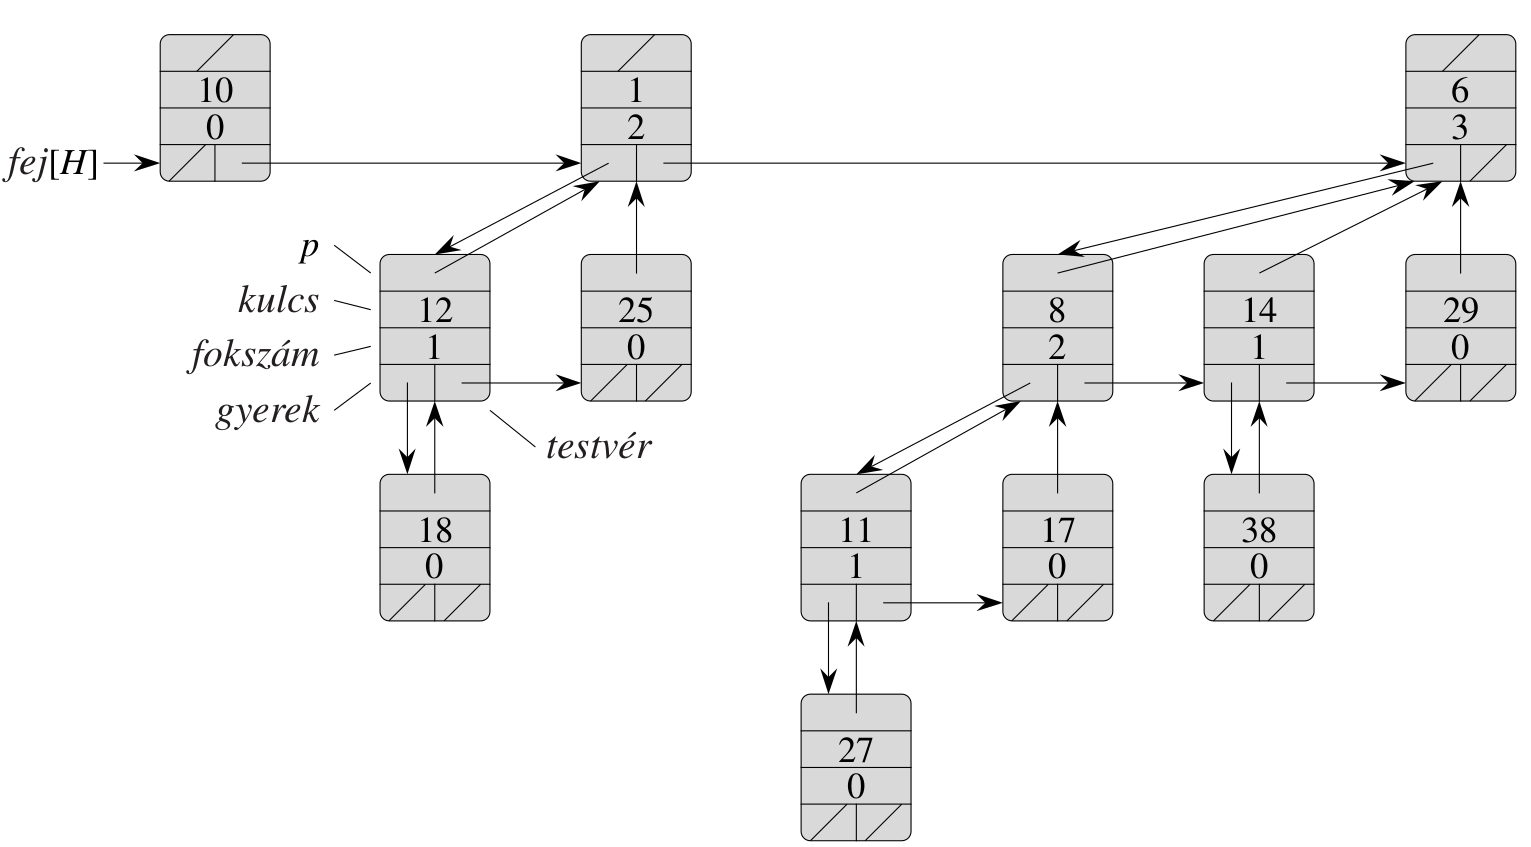
\includegraphics[width=\linewidth]{binom_heap}
\end{figure}

\framenote{Forrás: CLRS: Új algoritmusok 19.3~ábrája}
\end{frame}

\begin{frame}[fragile]{Minimális kulcs keresése}
	\begin{columns}
		\begin{column}{.6\linewidth}
\begin{alltt}
{\scshape BinomiálisKupacbanMin}(H) \{
   y = Nil
   x = H.fej //gyökérlista kezdőeleme
   min = Inf
   
   while (x != Nil) \{
      if (x.kulcs < min) \{
         min = x.kulcs
         y = x
      \}
      x = x.testver
   \}
   return y
 \}
\end{alltt}
		\end{column}
		\begin{column}<2>{.35\linewidth}
			$n$ kulcs esetén $O(\log{n})$
		\end{column}
	\end{columns}
\end{frame}

\begin{frame}{Kupacok egyesítése}
	\begin{itemize}
		\item $H_1, H_2$ bináris kupacok nem egyesíthetők hatékonyan, 
		binomiális kupacra azonban $O(\log{n})$ algoritmus adható
		\item Alapötlet
		\begin{itemize}
			\item Fokszám szerint nemcsökkenő sorrendben fűzzük össze a 
			$H_1$-ben és $H_2$-ben található binomiális fákat
			\begin{itemize}
				\item Legfeljebb $\log{n_1}+1 + \log{n_2}+1 \leq 2 \log{n} 
 +2=O(\log{n})$ hosszú listát kapunk
			\end{itemize}
			\item 2 darab $k$ fokszámú binomiális fából egy darab $k+1$ 
			fokszámú binomiális fa hozható létre (ennek ideje $O(1)$)
			\item Számoljuk föl az összefűzött gyökérlistában a megegyező 
			fokszámú binomiális fákat $\Rightarrow O(\log{n})$
		\end{itemize}
	\end{itemize}
\end{frame}

\begin{frame}{Kupacba történő beszúrás}

\begin{block}{Észrevétel}
A beszúrás két binomiális kupac egyesítéseként fogható föl, ahol az egyik 
binomiális kupacot alkotó egyedüli binomiális fa $B_0$.
\end{block}

\begin{example}<2>
	$\textcolor{red}{B_0-B_2-B_3} + \textcolor{blue}{B_0-B_1} \Rightarrow$ \\ 
	$\textcolor{red}{B_0}-\textcolor{blue}{B_0}-\textcolor{blue}{B_1}-\textcolor{red}{B_2}-\textcolor{red}{B_3}
	\Rightarrow$ \\
	$\textcolor{purple}{B_1}-\textcolor{blue}{B_1}-\textcolor{red}{B_2}-\textcolor{red}{B_3}\Rightarrow$
	 \\
	$B_2-\textcolor{red}{B_2}-\textcolor{red}{B_3} \Rightarrow$ \\
	$B_4 $
\end{example}
\end{frame}

\begin{frame}{Minimális kulcsú csúcs kivágása}
\begin{block}{Észrevételek}
	\begin{itemize}
		\item A minimális kulcsnak a gyökérlistában kell lennie $\Rightarrow 
		O(\log{n})$
		\item $B_k$ gyökérelemének eltávolítása után $k$ darab 
		szigorúan monoton csökkenő fokszámú binomiális 
		fára ``hullik szét''
	\end{itemize}
\end{block}

\begin{block}{Ötlet}
	\begin{itemize}
		\item A minimális kulcs eltávolítása után kapott $k$ binomiális fát 
		``fűzzük össze'' egy binomiális kupaccá, és azt egyesítsük az eredeti 
		kupaccal
	\end{itemize}
\end{block}
\end{frame}

\begin{frame}{Minimális kulcsú csúcs kivágása -- példa}
\begin{block}{Észrevételek}
	\begin{itemize}
		\item A minimális kulcsnak a gyökérlistában kell lennie $\Rightarrow 
		O(\log{n})$
		\item $B_k$ gyökérelemének eltávolítása után $k$ darab 
		szigorúan monoton csökkenő fokszámú binomiális 
		fára ``hullik szét''
	\end{itemize}
\end{block}
\begin{columns}[T]
	\begin{column}{.3\linewidth}
    \begin{tikzpicture}
[-,thick,every node/.style={shape=circle,inner 
	sep=1pt,draw,thick,minimum width=0.6cm}]
\node (a) at (0,0) {9};
%%
\node[fill=red] (b) at (1.5,0) {7}
child {node {14}
	child {node at (0,0) {21}}
}
child {node at (-.75,0) {11}
};
\path
\foreach \startNode/\endNode in {a/b}
{
	(\startNode) edge[-,thick] (\endNode)
};
\end{tikzpicture}
	\end{column}
	\begin{column}{.3\linewidth}
    \begin{tikzpicture}
[-,thick,every node/.style={shape=circle,inner 
	sep=1pt,draw,thick,minimum width=0.6cm}]
\node (a) {9};
\node[right of=a] (b) {14}
child {node {21}};
\node[right of=b] (c) {11};
\path (b) edge[-,thick] (c);
\end{tikzpicture}
	\end{column}
	\begin{column}{.3\linewidth}
		\begin{tikzpicture}
		[-,thick,every node/.style={shape=circle,inner 
			sep=1pt,draw,thick,minimum width=0.6cm}]
		\node at (1.5,0) {9}
		child {node {14}
			child {node at (0,0) {21}}
		}
		child {node at (-.75,0) {11}
		};
		\end{tikzpicture}
	\end{column}
\end{columns}
\end{frame}

\begin{frame}{Csúcsban kulcsának csökkentése/csúcs törlése}
\begin{block}{Kulcs csökkentése}
	\begin{itemize}
		\item Az adott csúcsban tárolt kulcsot csökkentsük a kívánt értékre 
		\pause $\rightarrow$ bináris kupacoknál megszokott módon javítsunk
	\end{itemize}
\end{block}

\begin{block}{Kulcs törlése}
	\begin{itemize}
		\item A törölni kívánt csúcsot kulcsát alkalmasan kicsire választjuk
		\pause $\rightarrow$ vágjuk ki a minimális kulcsot
	\end{itemize}
\end{block}

\begin{columns}
	\begin{column}{.2\linewidth}
		\begin{tikzpicture}
		[-,thick,every node/.style={shape=circle,inner 
			sep=1pt,draw,thick,minimum width=0.6cm}]
		\node (a) at (0,0) {9};
		\node (b) at (1.5,0) {7}
		child {node {14}
			child {node[fill=red] at (0,0) {21}}
		}
		child {node at (-.75,0) {11}
		}
		;
		\path
		\foreach \startNode/\endNode in {a/b}
		{
			(\startNode) edge[-,thick] (\endNode)
		};
		\end{tikzpicture}
	\end{column}
	\begin{column}{.2\linewidth}
		\begin{tikzpicture}
[-,thick,every node/.style={shape=circle,inner 
	sep=1pt,draw,thick,minimum width=0.6cm}]
\node (a) at (0,0) {9};
\node (b) at (1.5,0) {7}
child {node {14}
	child {node[fill=red] at (0,0) {0}}
}
child {node at (-.75,0) {11}
}
;
\path
\foreach \startNode/\endNode in {a/b}
{
	(\startNode) edge[-,thick] (\endNode)
};
\end{tikzpicture}
	\end{column}
\pause
	\begin{column}{.2\linewidth}
		\begin{tikzpicture}
[-,thick,every node/.style={shape=circle,inner 
	sep=1pt,draw,thick,minimum width=0.6cm}]
\node (a) at (0,0) {9};
\node[fill=red] (b) at (1.5,0) {0}
child {node {7}
	child {node at (0,0) {14}}
}
child {node at (-.75,0) {11}
}
;
\path
\foreach \startNode/\endNode in {a/b}
{
	(\startNode) edge[-,thick] (\endNode)
};
		\end{tikzpicture}
	\end{column}
	\begin{column}{.2\linewidth}
		\begin{tikzpicture}
[-,thick,every node/.style={shape=circle,inner 
	sep=1pt,draw,thick,minimum width=0.6cm}]
\node at (1.5,0) {7}
child {node {9}
	child {node at (0,0) {11}}
}
child {node at (-.75,0) {14}
}
;
\end{tikzpicture}
\end{column}
\end{columns}
\end{frame}

\begin{frame}{Bináris vs. binomiális kupac}
Kupacműveletek legrosszabb esetbeli viselkedése
\begin{table}
	\begin{tabular}{l|cc}
		Művelet   &   Bináris   &   Binomiális    \\ \hline
		{\rmfamily\scshape Min-keres} & $O(1)$ &  $O(\log{n})$ \\
		{\rmfamily\scshape Sorbol-Min} & $O(\log{n})$ &  $O(\log{n})$ \\
		{\rmfamily\scshape Beszúr}    & $O(\log{n})$ & $O(\log n)$ 
		\footnote{amortizált költségben 
		$O(1)$} \\
		{\rmfamily\scshape KulcsotCsökkent} & 	$O(\log{n})$ & $O(\log{n})$ \\
		{\rmfamily\scshape Egyesít} & $O(n)$ & $O(\log{n})$ \\
		{\rmfamily\scshape Töröl} & $O(\log{n})$ & $O(\log{n})$
		\\
	\end{tabular}
\end{table}
\end{frame}

\begin{frame}{Összegzés}
	\begin{itemize}
		\item Kupacokkal prioritási sorokat valósíthatunk meg hatékonyan
		\item Tetszőleges kulcs hatékony keresését nem támogatja
		\item Ha egyesíteni is akarunk kupacokat, akkor a binomiális kupac jobb 
		választás
			\begin{itemize}
				\item Igaz ekkor a {\rmfamily\scshape Min-keres} hatékonyságán 
				bukunk
			\end{itemize}
	\end{itemize}
\end{frame}

\end{document}